\documentclass{article}
\usepackage[english]{babel}
\usepackage{longtable}
\usepackage[top=1in, bottom=0.25in, left=1.25in, right=1.25in,includefoot,heightrounded]{geometry}
\usepackage{indentfirst}
\usepackage[utf8]{inputenc}
\usepackage{amsmath,amssymb}
\usepackage{graphicx,tikz}
\usepackage{hyperref}
\usepackage[colorinlistoftodos]{todonotes}
\usepackage[document]{ragged2e}
\usepackage{fancyhdr}
\usepackage{enumerate}
\usepackage{listings}
\usepackage{color}
\usepackage{flowchart}
\usepackage{hyperref}
\usetikzlibrary{arrows}

\usetikzlibrary{shapes.geometric, arrows}
\tikzstyle{startstop} = [rectangle, rounded corners, minimum width=3cm, minimum height=1cm,text centered, draw=black, fill=red!30]
\tikzstyle{decision} = [diamond, minimum width=4cm, minimum height=0.5cm, text centered, draw=black, fill=green!30]
\tikzstyle{process} = [rectangle, minimum width=3cm, minimum height=1cm, text centered, draw=black, fill=orange!30]
\tikzstyle{arrow} = [thick,->,>=stealth]
\tikzstyle{io} = [trapezium, trapezium left angle=70, trapezium right angle=110, minimum width=2cm, text width=4cm, minimum height=1cm, text centered, draw=black, fill=blue!30]

\pagestyle{fancy}
\fancyhf{}
\lhead{Myles Deslippe}
\rhead{Comp 3300 | Operating System Fundamentals}
\cfoot{\thepage}

\definecolor{MyDarkGreen}{rgb}{0.0,0.4,0.0}
\lstset{inputencoding=ansinew}
\lstset{breaklines=true} 

\begin{document}

    \section*{\centering{Processes}}

    \subsection*{Process Overview}
    \begin{itemize}
        \item A \textbf{process} is the instance of a \textbf{computer program} that is being executed by the \textbf{processor}.
        \item \textbf{Processes} are located in the system's \textbf{primary memory}, and are composed of:
        \begin{enumerate}
            \item The process text (executable instructions).
            \item The process data (global and static variables).
            \item The process heap (dynamically allocated memory).
            \item The process stack (local variables and function calls).
            \item The process state (managed by the kernel).
        \end{enumerate}
        \item[] \centering{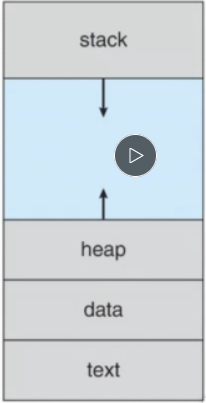
\includegraphics[height=150px]{images/Process.png}} 
        \item \raggedright Each \textbf{process' memory} is \textbf{isolated}, meaning it \textbf{cannot be accessed} by \textbf{other processes} (other than the kernel).
        \begin{itemize}
            \item This isolation is automatically enforced by the operating system.
            \item One bennifit of isolation, is the ability to limit the reach of malicious processes.
        \end{itemize}
        \item \textbf{Processes} may be composed of \textbf{several threads} allowing for \textbf{several instructions to be executed simultaneously}.
    \end{itemize}

    \subsection*{Process--Kernel Communication}
    \begin{itemize}
        \item \textbf{Processes} are not able to \textbf{directly access the kernel's memory}. Instead they use system calls, which interrupt the kernel, and indicate that a process requires a service.
        \item The \textbf{kernel} can access all \textbf{process'} memory.
    \end{itemize}

    \subsection*{Sharing the CPU}
    \begin{itemize}
        \item When \textbf{several processes} are running, system \textbf{resources need to be shared}.
        \item \textbf{Multiprogramming Operating Systems} \textbf{run processes} until they \textbf{block for an event}, when processes block for an event, they are \textbf{placed in a queue}, and the operating system executes \textbf{other processes}.
        \begin{itemize}
            \item This scheduling technique is bad because it could result in starvation if one process runs into an infinite loop.
        \end{itemize}
        \item \textbf{Time Sharing Operating Systems} give each \textbf{process} a \textbf{specific amount of time} to execute, and then \textbf{switch to the next}.
        \begin{itemize}
            \item This scheduling technique improves performance, and prevents starvation.
            \item This scheduling technique also gives the illusion that each process is running concurrently.
        \end{itemize}
    \end{itemize}

    \subsection*{Sharing Memory}
    \begin{itemize}
        \item Each process gets it's own \textbf{memory map}, which tells the \textbf{kernel} what memory belongs to the \textbf{process}.
        \item The \textbf{single contiguous memory model} is a model where the \textbf{RAM is occupied by one process at a time}. When that process completes, another is loaded.
        \begin{itemize}
            \item This model limits the size of processes to the maximum amount of RAM, and can only execute one process at a time.
        \end{itemize}
        \item The \textbf{partition model} allows \textbf{multiple processes} to \textbf{occupy} the RAM \textbf{simultaneously}.
        \begin{itemize}
            \item As long as sufficient contiguous memory is available, new processes are allocated memory.
            \item This model uses a partition table, that contains information about the allocated and unallocated memory (size, location, process occupying it).
            \item The operating system should detect unallocated contiguous memory blocks, and merge them into one large block. This has a lot of overhead, and leads to poor performance.
        \end{itemize}
        \item Modern operating systems use \textbf{virtual memory}, and \textbf{segmentation.}
        \begin{itemize}
            \item \textbf{Virtual memory} splits ram into \textbf{fixed size partitions} called \textbf{page frames} (typically 4KB).
            \item A \textbf{process} is \textbf{split} into \textbf{blocks of equal size} (block size = page frame size). Each block is numbered increamentally, however, the page frame they correspond to may or may not be consecutive.
            \item \textbf{Each process} is given a \textbf{page table}, that maps \textbf{blocks} to \textbf{actual page frames}.
            \item The processor \textbf{does not need to include all blocks} of a process in memory when it runs, only the ones that are required. It can \textbf{load} and \textbf{unload} them. 
        \end{itemize}
    \end{itemize}

    \subsection*{Process Control Block}
    \begin{itemize}
        \item The \textbf{process control block (PCB)} contains information associated with a \textbf{single process}.
        \item The PCB contains:
        \begin{enumerate}
            \item The \textbf{process state} (running, waiting, etc).
            \item The \textbf{program counter} (location of the next instruction to execute).
            \item \textbf{CPU register} values.
            \item \textbf{CPU scheduling information} (priorities, queue pointers).
            \item \textbf{Memory management information} (memory allocated to the process).
            \item \textbf{Accounting information} (CPU used, clock time since start, time limits).
            \item \textbf{I/O status information} (devices allocated to the process, file descriptors, etc). 
        \end{enumerate}
    \end{itemize}

    \subsection*{Process State Diagram}
    \begin{center}
        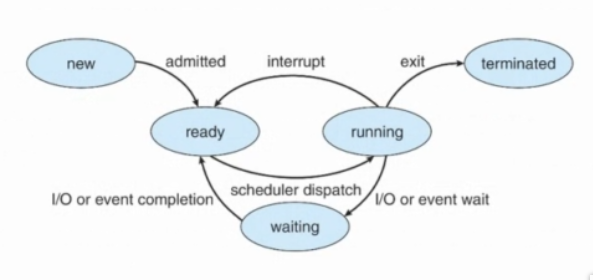
\includegraphics[width=300px]{images/Process-State-Diagram.png}
    \end{center}

    \subsection*{Process Creation}
    \begin{itemize}
        \item \textbf{Processes} are created from \textbf{forking}, which forms a \textbf{tree of processes} as more processes call fork.
        \item The \textbf{main process} (PID 1) is the process that is responsible for \textbf{managing the operating system}.
        \item \textbf{Copy on Write (COW)} | Initally, when fork is called \textbf{the pages are shared}. When data in the \textbf{shared pages change}, the OS \textbf{makes a copy of the page}, resulting in the child and the parent process having different copies of the specific page that changed.
    \end{itemize}

    \subsection*{Kernel Process Data}
    \begin{itemize}
        \item The kernel maintains a \textbf{page table}, a \textbf{process control block (PCB)}, and a \textbf{kernel stack} for each process.
        \item When a \textbf{process forks}, the \textbf{new child process will contain a clone of the parents data}. This data will have minor differences (pid, page table, etc).
        \begin{center}
            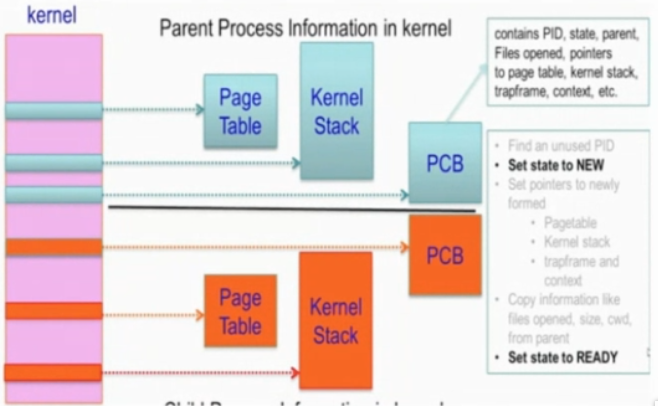
\includegraphics[width=300px]{images/Fork.png}
        \end{center}
    \end{itemize}

    \subsection*{Process Scheduling}
    \begin{itemize}
        \item \textbf{Process scheduling} is the way an \textbf{operating system} determines what \textbf{process' instructions} should be executed on a \textbf{CPU core}.
        \item The \textbf{goal of process scheduling} is to \textbf{maximize CPU use}, and \textbf{quickly switch between processes}.
        \item The \textbf{ready queue} is a queue of \textbf{processes} already in the main memory, that are \textbf{in the ready state}.
        \item The \textbf{process scheduler} takes \textbf{processes from the queue, and executes them}.
        \item The \textbf{scheduler} is triggered when a \textbf{timer interrupt occurs} or when a \textbf{process blocks for IO}. The \textbf{scheduler} will perform a \textbf{context switch} and start executing \textbf{another process}.
        \begin{center}
            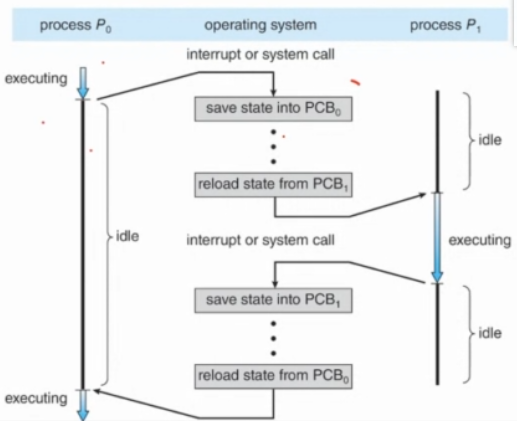
\includegraphics[width=300px]{images/Context-Switch.png}
        \end{center}
    \end{itemize}

    \subsection*{Process Termination}
    \begin{itemize}
        \item The \textbf{exit} system call returns an exit status to the \textbf{parent process}, which can be retrieved by the parent process by the \textbf{wait} system call.
        \begin{itemize}
            \item When the \textbf{wait} system call is invoked, the parent goes into a \textbf{blocked state} until one of it's \textbf{children terminate}. If there are no children, -1 is returned.
        \end{itemize}
        \item After \textbf{exit} is invoked, the process' resources are \textbf{deallocated by the operating system}.
        \item The \textbf{parent process} may \textbf{terminate the execution} of \textbf{itsself and/or it's child processes} with the \textbf{abort} system call.
        \begin{itemize}
            \item This may be done if the child has exceeded allocated resources, the child's task is no longer required, or the parent is exiting.
        \end{itemize}
    \end{itemize}

    \subsection*{Zombie Processes and Orphan Processses}
    \begin{itemize}
        \item When a \textbf{process terminates} it \textbf{still exists} in the operating system to allow the \textbf{parent process} to read the \textbf{child process' exiy status}. When a child process is in such a state, it is referred to as a \textbf{zombie process}.
        \item When the \textbf{parent process} reads the \textbf{child process' status} the zombie process is removed.
        \item If the \textbf{parent never} invokes the \textbf{wait} system call, the \textbf{zombie process} will exist \textbf{infinitely} (which is a resource leak).
        \item An \textbf{orphan process} is a process whose \textbf{parent has termated} before it.
        \item When a \textbf{process' parent termates before it}, it is \textbf{adopted by the first process (init process)}.
    \end{itemize}

    \section*{Interprocess Communication}

    \subsection*{Process Concepts}
    \begin{itemize}
        \item \textbf{Each process} can only view \textbf{its virtual address}. It \textbf{cannot view others}, and \textbf{cannot determine the physical address mapping}.
        \item \textbf{Processes} within a system may be \textbf{independent} or \textbf{cooperating}.
        \item \textbf{Cooperating processes} can \textbf{affect} or be \textbf{affected} by \textbf{other processes}.
        \item Reasons for \textbf{cooperating processes} include:
        \begin{enumerate}
            \item Information sharing.
            \item Computation speed increase.
            \item Modularity.
            \item Convenience.
        \end{enumerate}
        \item \textbf{Cooperating processes} need \textbf{interprocess communication (IPC)}.
        \item There are two \textbf{models} of \textbf{IPD}: \textbf{shared memory}, and \textbf{message passing}.
    \end{itemize}

    \subsection*{IPC Shared Memory}
    \begin{itemize}
        \item \textbf{IPC shared memory} involves \textbf{allocating memory} that \textbf{several processes can access}.
        \item In this model, the \textbf{communication} is under the control of the \textbf{user's processes} not the \textbf{operating system}.
        \item This model is \textbf{fast}, but it is \textbf{very difficult} to provice a mechanism that will allow the \textbf{user's process} to \textbf{synchronize their actions}.
        \item[] \begin{center}
                    \includegraphics*[height=150px]{images/Shared-Memory.PNG}
                \end{center} 
    \end{itemize}

    \subsection*{IPC Message Passing}
    \begin{itemize}
        \item \textbf{IPC message passing} uses \textbf{shared memory} created \textbf{in the kernel}.
        \item \textbf{Processes} then use system calls to \textbf{send}, and \textbf{receive data}.
        \item This is \textbf{slower}, but allows for \textbf{processes} to easily \textbf{synchronize their communication}.
        \item[] \begin{center}
            \includegraphics*[height=150px]{images/Message-Passing.PNG}
        \end{center} 
    \end{itemize}

    \subsection*{Pipes}
    \begin{itemize}
        \item To allow \textbf{two processes} to \textbf{communicate} using \textbf{message passing}, we use \textbf{pipes} to establish a \textbf{communication link}.
        \item A \textbf{parent process} creates a pipe via the \textbf{fork} function, and can use it to communicate with \textbf{child processes}. 
        \begin{itemize}
            \item The pipe must be created before the child process.
        \end{itemize}
        \item \textbf{Pipes} are \textbf{unidirectional communication channels}  that consist of two file descriptors: \textbf{read} and \textbf{write} respectively. 
    \end{itemize}

    \subsection*{Named Pipes}
    \begin{itemize}
        \item \textbf{Named pipes} are \textbf{more powerful} than \textbf{ordinary pipes}.
        \item \textbf{Named pipes} allow for \textbf{bidirectional communication}, and can be used by \textbf{more than two processes}.
        \item \textbf{Named pipes} also do not require a \textbf{parent-child relationship} to establish communication.
    \end{itemize}

    \subsection*{Sockets}
    \begin{itemize}
        \item A \textbf{socket} is a \textbf{communication endpoint}.
        \item \textbf{Sockets} are \textbf{bidirectional communication channels} that allow \textbf{two processes} to communicate \textbf{over a network}.
        \item \textbf{Sockets} use \textbf{ports} which are \textbf{bound to file descriptors} to enable communication.
        \item All \textbf{ports below 1024} are \textbf{well-known ports} that are used for standard services.
    \end{itemize}

    \subsection*{Remote Procedure Calls}
    \begin{itemize}
        \item \textbf{Remote Procedure Calls (RPC)} abstracts \textbf{procedure calls} between \textbf{processes} on \textbf{networked systems}.
        \item \textbf{RPC} uses \textbf{sockets for communication}.
    \end{itemize}

\end{document}
